\newpage
\section{Progetto Hardware e Documentazione Tecnica}
\label{appendix:hardware}

In questa appendice vengono sintetizzati brevemente i dettagli costruttivi del sistema, includendo gli schemi elettrici principali, le scelte relative al layout del PCB e la distinta dei componenti (BOM).

\subsection{Schemi Elettrici}
Il design è stato suddiviso in blocchi funzionali per garantire la modularità e facilitare il debugging. Di seguito vengono riportati i circuiti principali:

\subsubsection*{Sottosistema di Elaborazione e Memoria}
Include il SoC Raspberry Pi RP2040, il circuito di clock a \qty{12}{MHz}, il pulsante di \textit{Reset} e la memoria Flash W25Q16 collegata tramite bus QSPI.
\begin{figure}[H]
     \centering
     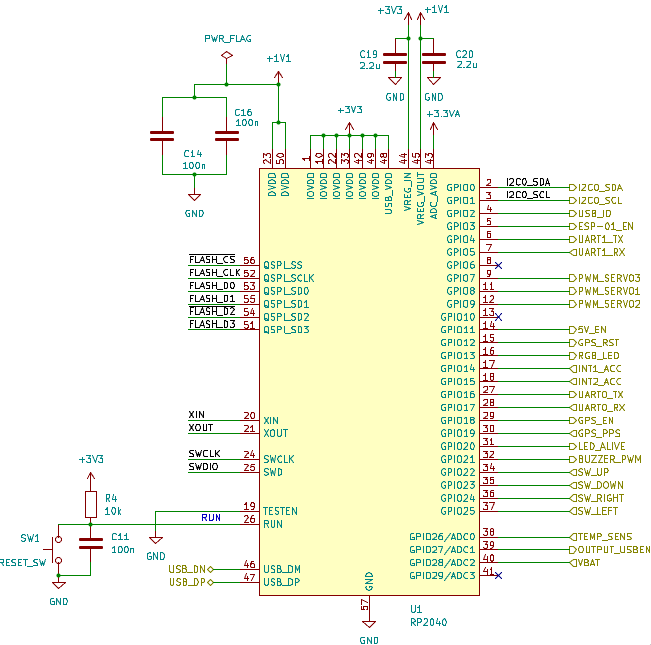
\includegraphics[width=0.6\linewidth]{media/schematic/schematic_mcu.png}
     \caption{Schema elettrico del core RP2040 e periferiche di supporto.}
\end{figure}

\subsubsection*{Sottosistema GNSS e RF}
Circuito di interfaccia del modulo u-blox SAM-M8Q, comprensivo di filtraggio dell'alimentazione dedicato e connessione UART verso l'MCU.
\begin{figure}[H]
     \centering
     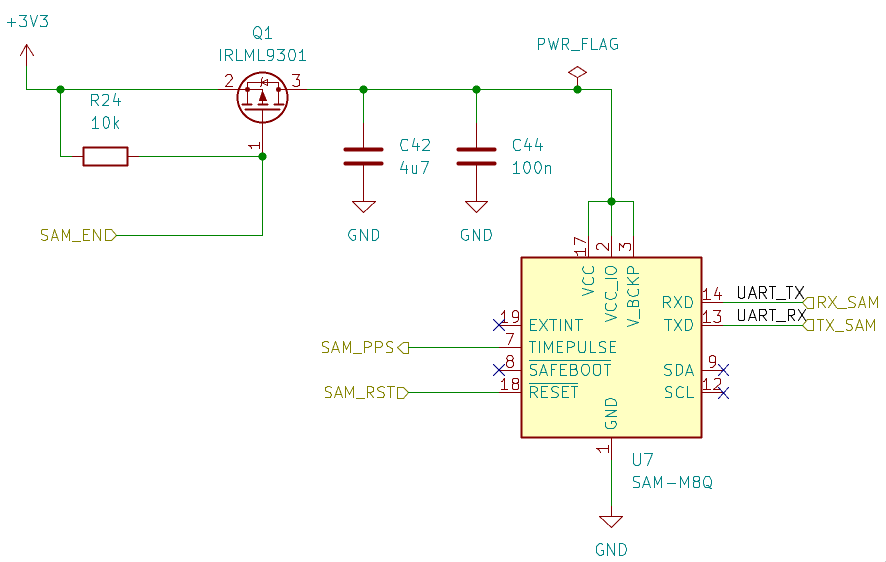
\includegraphics[width=0.6\linewidth]{media/schematic/schematic_gnss.png}
     \caption{Schema del modulo GNSS e sezione antenna.}
     \label{fig:gps_schematic}
\end{figure}

\subsubsection*{Buck converter}
\begin{figure}[H]
    \centering
    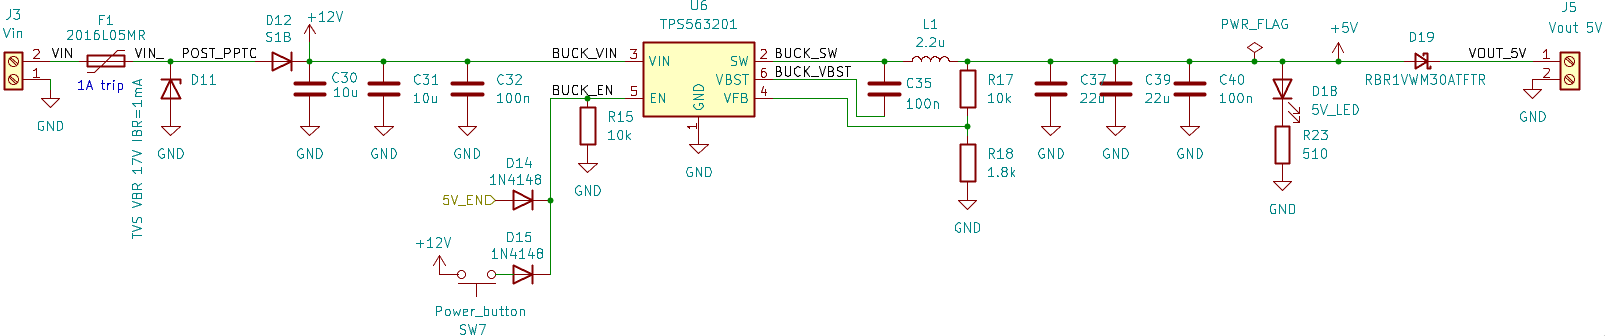
\includegraphics[width=0.8\linewidth]{media/schematic/schematic_buck.png}
    \caption{Schema circuitale del convertitore DC-DC buck per la linea di potenza a \qty{5}{V}.}
    \label{fig:buck_schematic}
\end{figure}

\subsubsection*{LDO}
\begin{figure}[H]
    \centering
    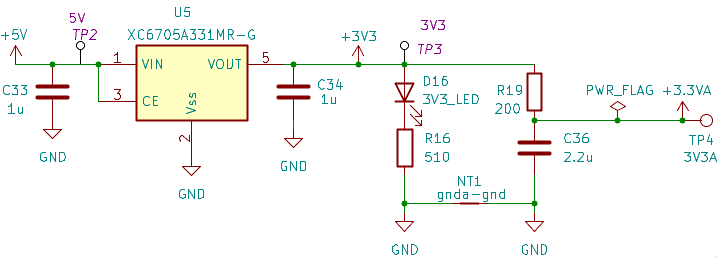
\includegraphics[width=0.6\linewidth]{media/schematic/schematic_ldo.png}
    \caption{Stadio di regolazione lineare per l'alimentazione della logica e del modulo GNSS.}
    \label{fig:ldo_schematic}
\end{figure}

\subsubsection*{Pulsanti}
\begin{figure}[H]
    \centering
    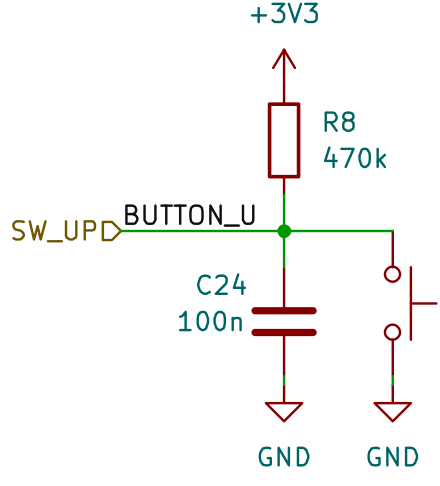
\includegraphics[width=0.3\linewidth]{media/schematic/schematic_button.png}
    \caption{Schematico dei pulsanti: rete RC e Pull-up interno.}
    \label{fig:button_sch}
\end{figure}

\subsubsection*{Flash}
\begin{figure}[H]
    \centering
    % 
    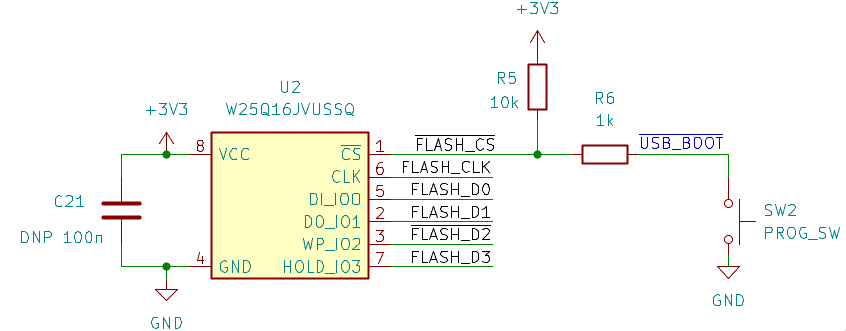
\includegraphics[width=0.7\linewidth]{media/schematic/schematic_flash.png} 
    \caption{Circuito di interfaccia QSPI tra RP2040 e memoria Flash \cite{w25q128_ds}.}
    \label{fig:flash_schematic}
\end{figure}